%!tex program = lualatex
\documentclass{ctexart}
\usepackage{amsmath, amssymb}
\usepackage{enumitem}
\usepackage{xcolor}
\usepackage{pgfplots}
\pgfplotsset{compat=1.18}
\ctexset{
  section/name = {问题},
  section/nameformat += {\sffamily},
  section/numberformat += {\color{magenta}\Huge}
}
%%%%%%%%%%%%%%%%%%%%%%%%%%%%%%%%%%%%%%%%%%%%%%%%%%%%%%%%%%%%%%%%%%%%%%%%%%%%%%%
\usepackage[most]{tcolorbox}
\usetikzlibrary{arrows.meta}
%%%%%%%%%%%%%%%%%%%%%%%%%%%%%%%%%%%%%%%%%%%%%%%%%%%%%%%%%%%%%%%%%%%%%%%%%%%%%%%
\usepackage{algorithm}
\usepackage{algpseudocodex}
\usepackage{caption}
\captionsetup[algorithm]{name={算法}}
%%%%%%%%%%%%%%%%%%%%%%%%%%%%%%%%%%%%%%%%%%%%%%%%%%%%%%%%%%%%%%%%%%%%%%%%%%%%%%%
\usepackage{silence}
\WarningFilter{latexfont}{Font shape}
\WarningFilter{latexfont}{Size substitutions}
\WarningFilter{latexfont}{Some font}
\hfuzz=15pt
%%%%%%%%%%%%%%%%%%%%%%%%%%%%%%%%%%%%%%%%%%%%%%%%%%%%%%%%%%%%%%%%%%%%%%%%%%%%%%%
\usepackage{hyperref}
\hypersetup{
  colorlinks = true,
  urlcolor = magenta,
  linkcolor = cyan
}
%%%%%%%%%%%%%%%%%%%%%%%%%%%%%%%%%%%%%%%%%%%%%%%%%%%%%%%%%%%%%%%%%%%%%%%%%%%%%%%
\newcommand{\red}[1]{\textcolor{red}{#1}}
%%%%%%%%%%%%%%%%%%%%%%%%%%%%%%%%%%%%%%%%%%%%%%%%%%%%%%%%%%%%%%%%%%%%%%%%%%%%%%%
\usepackage{siunitx}
\sisetup{
  group-separator = {,},
}
%%%%%%%%%%%%%%%%%%%%%%%%%%%%%%%%%%%%%%%%%%%%%%%%%%%%%%%%%%%%%%%%%%%%%%%%%%%%%%%
\begin{document}
\chapter{Multiples of 3 or 5}
\section{Description}
If we list all the natural numbers below 10 that are multiples of 3 or 5, we get 3, 5, 6 and 9. The sum of these multiples is 23.

Find the sum of all the multiples of 3 or 5 below 1000.
试试看中文能不能显示?
\section{Flow Chart}

\begin{center}
	\begin{tikzpicture}[node distance=2cm]
		\node (start) [startstop] {开始};
		\node (in1) [io, right of=start, xshift=3cm] {输入一个上限cap};
		\node (pro1) [operation, right of=in1, xshift=3cm] {n = 1\\
			sum = 0};
		\node (dec1) [decision, below of=pro1, yshift=-1cm] {n能被3\\
			或者5整除};
		\node (pro2) [yshift=-1cm, operation, below of = dec1] {sum += n;\\
			++n;};
		\node (dec2) [decision, below of=pro2, yshift=-.5cm] {n < cap};
		\node (out1) [io, left of=dec2, xshift=-3cm] {输出数据};
		\node (stop) [startstop, left of=out1, xshift=-3cm] {终止};

		\draw [arrow] (start) -- (in1);
		\draw [arrow] (in1) -- (pro1);
		\draw [arrow] (pro1) -- (dec1);
		\draw [arrow] (dec1) -- node[anchor=east] {Yes}(pro2);
		\draw [arrow] (pro2) --  (dec2);
		\draw [arrow] (dec2.west) -- node[above] {No} (out1);
		\draw [arrow] (dec2.east) -| ([xshift=2cm]dec1.east) -- node[anchor=south east, text centered] {Yes} (dec1.east);
		\draw [arrow] (out1) -- (stop);
	\end{tikzpicture}
	\captionof{figure}{Multiples of 3 or 5}
\end{center}

\section{Codes}
\begin{cpp}
	long Solution::sum_of_multiples(int cap)
	{
			long sum{};

			for(int i{1}; i < cap; ++i)
			{
					if(i % 3 == 0 || i % 5 == 0) sum += i;
				}
			return sum;
		}
\end{cpp}

\section{title}
\subsection{Problem Description}
\begin{tcolorbox}

\end{tcolorbox}
		

\section{title}
\subsection{Problem Description}
\begin{tcolorbox}

\end{tcolorbox}
		

\section{title}
\subsection{Problem Description}
\begin{tcolorbox}

\end{tcolorbox}
		

\section{最小公倍数}\label{sec:problem05}
\subsection{问题描述}
\begin{tcolorbox}
	2520 是能够被 1 到 10 的每个数字整除的最小数字。

	求最小的正整数,使得它能够被 1 到 20 的每个数字整除。
\end{tcolorbox}

\subsection{算法}
最大公约数在STL中有提供,但是做为数学及编程的最基本的内容,还是有必要自己写一下的。

\textbf{数学原理}:

欧几里得算法基于这样一个定理:两个整数  $ a $  和  $ b $  的最大公约数等于  $b$  和 \( a \mod b \) 的最大公约数,其中 \(
a \mod b \) 是  $a$  除以  $b$  的余数。

\begin{algorithm}
	\caption{最大公约数}
	\begin{algorithmic}[1]
		\Function{Gcd}{$a, b$}
		\While{b \neq 0}
		\State $ temp = a$
		\State $ a = b$
		\State $ b = temp \mod b$
		\EndWhile
		\Return $a$
		\EndFunction
	\end{algorithmic}
\end{algorithm}

\begin{algorithm}
	\caption{最小公倍数}
	\begin{algorithmic}[1]
		\Function{Lcm}{$a, b$}
			\If{$a = 0 \text{ or } b = 0$}
				\Return $0$
			\EndIf
			\Return $\left|\frac{a \times b}{\text{gcd}(a,b)}\right|$
		\EndFunction
	\end{algorithmic}
\end{algorithm}

\subsection{答案}
232792560

\section{平方和之差}
\subsection{问题描述}
\begin{tcolorbox}
	前十个自然数的平方和是:

	\[
		1^2 + 2^2 + \dots + 10^2 = 385
	\]

	前十个自然数的和的平方是:

	\[
		(1 + 2 + \dots + 10)^2 = 55^2 = 3025
	\]

	因此,和的平方与平方和之间的差为 \( 3025 - 385 = 2640 \)。

	请找到前 100 个自然数的和的平方与平方和之间的差。
\end{tcolorbox}

\subsection{答案}
 25164150

\section{第10001个质数}
\subsection{问题描述}
\begin{tcolorbox}
通过列出前六个质数:2, 3, 5, 7, 11 和 13,可以看到第六个质数是 13。

求第 10001 个质数是多少?
\end{tcolorbox}

\subsection{算法}

\subsection{答案}

\section{数列中的最大乘积}\label{sec:problem08}
\subsection{问题描述}
\begin{tcolorbox}
在下面这个 1000 位的数字中,相邻的四个数字的最大乘积是 9 × 9 × 8 × 9 = 5832。

\begin{verbatim}
73167176531330624919225119674426574742355349194934
96983520312774506326239578318016984801869478851843
85861560789112949495459501737958331952853208805511
12540698747158523863050715693290963295227443043557
66896648950445244523161731856403098711121722383113
62229893423380308135336276614282806444486645238749
30358907296290491560440772390713810515859307960866
70172427121883998797908792274921901699720888093776
65727333001053367881220235421809751254540594752243
52584907711670556013604839586446706324415722155397
53697817977846174064955149290862569321978468622482
83972241375657056057490261407972968652414535100474
82166370484403199890008895243450658541227588666881
16427171479924442928230863465674813919123162824586
17866458359124566529476545682848912883142607690042
24219022671055626321111109370544217506941658960408
07198403850962455444362981230987879927244284909188
84580156166097919133875499200524063689912560717606
05886116467109405077541002256983155200055935729725
71636269561882670428252483600823257530420752963450
\end{verbatim}

找出这个 1000 位数字中,相邻的 13 个数字的乘积最大的值。这个最大的乘积是多少?
\end{tcolorbox}

\subsection{算法}
这道题比较简单,只要遍历即可。如果遇到0就直接跳到0后面的数字再开始。

需要注意的是这个算法中会用字符串来表示大数字,所以取出的数字是字符,需要做相应的运算才能成为数值。

\subsection{答案}
23514624000

\section{特殊勾股数}\label{sec:problem09}
\subsection{问题描述}
\begin{tcolorbox}
	一组勾股数是一组三个自然数 \( a < b < c \),使得:

	\[
		a^2 + b^2 = c^2
	\]

	例如,\( 3^2 + 4^2 = 9 + 16 = 25 = 5^2 \)。

	有且只有一组勾股数满足 \( a + b + c = 1000 \)。求出这组勾股数中 \( abc \) 的乘积。
\end{tcolorbox}

\subsection{算法}
这道题只需要遍历即可实现求解,值得考虑的地方是遍历的边界。因为三角形的一条边肯定小于另外两条边的和(勾股数可以看作直角三角形的三条边),所以斜边
\( c \) 最多不会超过499,而 \( a + b + c = 0, c > a, c > b \), 所以有 \( c \geqslant 334 \)。

\subsection{答案}
31875000

\section{质数之和}\label{sec:problem10}
\subsection{问题描述}
\begin{tcolorbox}
小于 10 的质数的和是 \(2 + 3 + 5 + 7 = 17\)。

请找出所有小于两百万的质数的和。
\end{tcolorbox}

\subsection{算法}
用问题\ref{sec:prime}中的筛法即可解决。

\subsection{答案}
142913828922

\section{矩阵中的最大乘积}
\subsection{问题描述}
\begin{tcolorbox}
	在下面这个 20×20 的网格中,沿对角线的四个相邻数字已经标记为红色,这些数字的乘积是 \(  26 \times 63 \times 78 \times 14 = 1788696 \) 。
	\begin{equation*}
		\begin{array}{@{\hspace{4pt}}c@{\hspace{4pt}}c@{\hspace{4pt}}c@{\hspace{4pt}}c@{\hspace{4pt}}c@{\hspace{4pt}}c@{\hspace{4pt}}c@{\hspace{4pt}}c@{\hspace{4pt}}c@{\hspace{4pt}}c@{\hspace{4pt}}c@{\hspace{4pt}}c@{\hspace{4pt}}c@{\hspace{4pt}}c@{\hspace{4pt}}c@{\hspace{4pt}}c@{\hspace{4pt}}c@{\hspace{4pt}}c@{\hspace{4pt}}c@{\hspace{4pt}}c}
			08 & 02 & 22 & 97 & 38 & 15 & 00 & 40 & 00                  & 75                  & 04                  & 05                  & 07 & 78 & 52 & 12 & 50 & 77 & 91 & 08 \\
			49 & 49 & 99 & 40 & 17 & 81 & 18 & 57 & 60                  & 87                  & 17                  & 40                  & 98 & 43 & 69 & 48 & 04 & 56 & 62 & 00 \\
			81 & 49 & 31 & 73 & 55 & 79 & 14 & 29 & 93                  & 71                  & 40                  & 67                  & 53 & 88 & 30 & 03 & 49 & 13 & 36 & 65 \\
			52 & 70 & 95 & 23 & 04 & 60 & 11 & 42 & 69                  & 24                  & 68                  & 56                  & 01 & 32 & 56 & 71 & 37 & 02 & 36 & 91 \\
			22 & 31 & 16 & 71 & 51 & 67 & 63 & 89 & 41                  & 92                  & 36                  & 54                  & 22 & 40 & 40 & 28 & 66 & 33 & 13 & 80 \\
			24 & 47 & 32 & 60 & 99 & 03 & 45 & 02 & 44                  & 75                  & 33                  & 53                  & 78 & 36 & 84 & 20 & 35 & 17 & 12 & 50 \\
			32 & 98 & 81 & 28 & 64 & 23 & 67 & 10 & \textcolor{red}{26} & 38                  & 40                  & 67                  & 59 & 54 & 70 & 66 & 18 & 38 & 64 & 70 \\
			67 & 26 & 20 & 68 & 02 & 62 & 12 & 20 & 95                  & \textcolor{red}{63} & 94                  & 39                  & 63 & 08 & 40 & 91 & 66 & 49 & 94 & 21 \\
			24 & 55 & 58 & 05 & 66 & 73 & 99 & 26 & 97                  & 17                  & \textcolor{red}{78} & 78                  & 96 & 83 & 14 & 88 & 34 & 89 & 63 & 72 \\
			21 & 36 & 23 & 09 & 75 & 00 & 76 & 44 & 20                  & 45                  & 35                  & \textcolor{red}{14} & 00 & 61 & 33 & 97 & 34 & 31 & 33 & 95 \\
			78 & 17 & 53 & 28 & 22 & 75 & 31 & 67 & 15                  & 94                  & 03                  & 80                  & 04 & 62 & 16 & 14 & 09 & 53 & 56 & 92 \\
			16 & 39 & 05 & 42 & 96 & 35 & 31 & 47 & 55                  & 58                  & 88                  & 24                  & 00 & 17 & 54 & 24 & 36 & 29 & 85 & 57 \\
			86 & 56 & 00 & 48 & 35 & 71 & 89 & 07 & 05                  & 44                  & 44                  & 37                  & 44 & 60 & 21 & 58 & 51 & 54 & 17 & 58 \\
			19 & 80 & 81 & 68 & 05 & 94 & 47 & 69 & 28                  & 73                  & 92                  & 13                  & 86 & 52 & 17 & 77 & 04 & 89 & 55 & 40 \\
			04 & 52 & 08 & 83 & 97 & 35 & 99 & 16 & 07                  & 97                  & 57                  & 32                  & 16 & 26 & 26 & 79 & 33 & 27 & 98 & 66 \\
			88 & 36 & 68 & 87 & 57 & 62 & 20 & 72 & 03                  & 46                  & 33                  & 67                  & 46 & 55 & 12 & 32 & 63 & 93 & 53 & 69 \\
			04 & 42 & 16 & 73 & 38 & 25 & 39 & 11 & 24                  & 94                  & 72                  & 18                  & 08 & 46 & 29 & 32 & 40 & 62 & 76 & 36 \\
			20 & 69 & 36 & 41 & 72 & 30 & 23 & 88 & 34                  & 62                  & 99                  & 69                  & 82 & 67 & 59 & 85 & 74 & 04 & 36 & 16 \\
			20 & 73 & 35 & 29 & 78 & 31 & 90 & 01 & 74                  & 31                  & 49                  & 71                  & 48 & 86 & 81 & 16 & 23 & 57 & 05 & 54 \\
			01 & 70 & 54 & 71 & 83 & 51 & 54 & 69 & 16                  & 92                  & 33                  & 48                  & 61 & 43 & 52 & 01 & 89 & 19 & 67 & 48
		\end{array}
	\end{equation*}
相邻(上下左右对角线)的四个数字乘积的最大值是多少?
\end{tcolorbox}

\subsection{算法}
遍历,注意边界。另外,也要考虑反对角线。

\subsection{答案}
70600674

\section{高度可被整除的三角形数}\label{sec:problem12}
\subsection{问题描述}
\begin{tcolorbox}
	三角形数序列是通过逐个加上自然数来生成的。也就是说,第七个三角形数是

	\[
		1 + 2 + 3 + 4 + 5 + 6 + 7 = 28
	\]

	前十个三角形数是:

	\[
		1, 3, 6, 10, 15, 21, 28, 36, 45, 55, \ldots
	\]


	前七个三角形数的约数为:
	\begin{align*}
		\mathbf 1   & \colon 1             \\
		\mathbf 3   & \colon 1,3           \\
		\mathbf 6   & \colon 1,2,3,6       \\
		\mathbf{10} & \colon 1,2,5,10      \\
		\mathbf{15} & \colon 1,3,5,15      \\
		\mathbf{21} & \colon 1,3,7,21      \\
		\mathbf{28} & \colon 1,2,4,7,14,28
	\end{align*}
	我们可以看到,28 的约数有:1, 2, 4, 7, 14, 28。
	第一个拥有超过五个约数的三角形数是 28。

	第一个拥有超过 500 个约数的三角形数是多少?
\end{tcolorbox}

\subsection{算法}
\begin{algorithm}[H]
	\caption{算法标题}
	\begin{algorithmic}[1]
	\Function{CountDivisors}{$N$}
	\State $root \gets \lfloor \sqrt{N} \rfloor$
	\State $ count \gets 0$
	\For{$i \gets 1$ to $root$}
	\State $count \gets count + 2$
	\EndFor
	\If{$root \times root = N$}
	\State $count \gets count - 1$
	\EndIf
	\Return $count$
	\EndFunction
	\end{algorithmic}
\end{algorithm}

\subsection{答案}
76576500

\section{大数加法}
\subsection{问题描述}
\begin{tcolorbox}[breakable]
下列是一百个 50 位的数字:

\begin{center}
37107287533902102798797998220837590246510135740250 \\
46376937677490009712648124896970078050417018260538 \\
74324986199524741059474233309513058123726617309629 \\
91942213363574161572522430563301811072406154908250 \\
23067588207539346171171980310421047513778063246676 \\
89261670696623633820136378418383684178734361726757 \\
28112879812849979408065481931592621691275889832738 \\
44274228917432520321923589422876796487670272189318 \\
47451445736001306439091167216856844588711603153276 \\
70386486105843025439939619828917593665686757934951 \\
62176457141856560629502157223196586755079324193331 \\
64906352462741904929101432445813822663347944758178 \\
92575867718337217661963751590579239728245598838407 \\
58203565325359399008402633568948830189458628227828 \\
80181199384826282014278194139940567587151170094390 \\
35398664372827112653829987240784473053190104293586 \\
86515506006295864861532075273371959191420517255829 \\
71693888707715466499115593487603532921714970056938 \\
54370070576826684624621495650076471787294438377604 \\
53282654108756828443191190634694037855217779295145 \\
36123272525000296071075082563815656710885258350721 \\
45876576172410976447339110607218265236877223636045 \\
17423706905851860660448207621209813287860733969412 \\
81142660418086830619328460811191061556940512689692 \\
51934325451728388641918047049293215058642563049483 \\
62467221648435076201727918039944693004732956340691 \\
15732444386908125794514089057706229429197107928209 \\
55037687525678773091862540744969844508330393682126 \\
18336384825330154686196124348767681297534375946515 \\
80386287592878490201521685554828717201219257766954 \\
78182833757993103614740356856449095527097864797581 \\
16726320100436897842553539920931837441497806860984 \\
48403098129077791799088218795327364475675590848030 \\
87086987551392711854517078544161852424320693150332 \\
59959406895756536782107074926966537676326235447210 \\
69793950679652694742597709739166693763042633987085 \\
41052684708299085211399427365734116182760315001271 \\
65378607361501080857009149939512557028198746004375 \\
35829035317434717326932123578154982629742552737307 \\
94953759765105305946966067683156574377167401875275 \\
88902802571733229619176668713819931811048770190271 \\
25267680276078003013678680992525463401061632866526 \\
36270218540497705585629946580636237993140746255962 \\
24074486908231174977792365466257246923322810917141 \\
91430288197103288597806669760892938638285025333403 \\
34413065578016127815921815005561868836468420090470 \\
23053081172816430487623791969842487255036638784583 \\
11487696932154902810424020138335124462181441773470 \\
63783299490636259666498587618221225225512486764533 \\
67720186971698544312419572409913959008952310058822 \\
95548255300263520781532296796249481641953868218774 \\
76085327132285723110424803456124867697064507995236 \\
37774242535411291684276865538926205024910326572967 \\
23701913275725675285653248258265463092207058596522 \\
29798860272258331913126375147341994889534765745501 \\
18495701454879288984856827726077713721403798879715 \\
38298203783031473527721580348144513491373226651381 \\
34829543829199918180278916522431027392251122869539 \\
40957953066405232632538044100059654939159879593635 \\
29746152185502371307642255121183693803580388584903 \\
41698116222072977186158236678424689157993532961922 \\
62467957194401269043877107275048102390895523597457 \\
23189706772547915061505504953922979530901129967519 \\
86188088225875314529584099251203829009407770775672 \\
11306739708304724483816533873502340845647058077308 \\
82959174767140363198008187129011875491310547126581 \\
97623331044818386269515456334926366572897563400500 \\
42846280183517070527831839425882145521227251250327 \\
55121603546981200581762165212827652751691296897789 \\
32238195734329339946437501907836945765883352399886 \\
75506164965184775180738168837861091527357929701337 \\
62177842752192623401942399639168044983993173312731 \\
32924185707147349566916674687634660915035914677504 \\
99518671430235219628894890102423325116913619626622 \\
73267460800591547471830798392868535206946944540724 \\
76841822524674417161514036427982273348055556214818 \\
97142617910342598647204516893989422179826088076852 \\
87783646182799346313767754307809363333018982642090 \\
10848802521674670883215120185883543223812876952786 \\
71329612474782464538636993009049310363619763878039 \\
62184073572399794223406235393808339651327408011116 \\
66627891981488087797941876876144230030984490851411 \\
60661826293682836764744779239180335110989069790714 \\
85786944089552990653640447425576083659976645795096 \\
66024396409905389607120198219976047599490197230297 \\
64913982680032973156037120041377903785566085089252 \\
16730939319872750275468906903707539413042652315011 \\
94809377245048795150954100921645863754710598436791 \\
78639167021187492431995700641917969777599028300699 \\
15368713711936614952811305876380278410754449733078 \\
40789923115535562561142322423255033685442488917353 \\
44889911501440648020369068063960672322193204149535 \\
41503128880339536053299340368006977710650566631954 \\
81234880673210146739058568557934581403627822703280 \\
82616570773948327592232845941706525094512325230608 \\
22918802058777319719839450180888072429661980811197 \\
77158542502016545090413245809786882778948721859617 \\
72107838435069186155435662884062257473692284509516 \\
20849603980134001723930671666823555245252804609722 \\
53503534226472524250874054075591789781264330331690 \\
\end{center}

这些数字的总和为多少?请只给出前十位数字。
\end{tcolorbox}

\subsection{算法}
这道题需要实现字符串数字的加法,为了以后方面,可以设计一个字符串数字的类。当然也可以借鉴Python中无限大整数的实现方式。

\subsection{答案}
5537376230

\section{最长考拉兹序列}
\subsection{问题描述}
\begin{tcolorbox}
考拉兹序列是这样定义的:

\begin{itemize}
    \item 对于任意正整数 $n$,如果 $n$ 是偶数,则下一项是 $n / 2$;
    \item 如果 $n$ 是奇数,则下一项是 $3n + 1$。
\end{itemize}

使用这个规则不断重复,最终序列会到达 1。例如,使用 13 生成的考拉兹序列如下:

\[
13 \to 40 \to 20 \to 10 \to 5 \to 16 \to 8 \to 4 \to 2 \to 1
\]

这个序列有 10 项。尽管尚未被证明(称为考拉兹猜想),但相信所有的起始数字最终都能到达 1。

哪一个起始数字,$n < 1,000,000$,能够生成最长的序列?
\end{tcolorbox}

\subsection{算法}
这道题只需要遍历即可。

\subsection{答案}

\section{格子路径}\label{sec:problem15}
\subsection{网格中的路径}
\begin{tcolorbox}
	从一个 $2 \times 2$网格的左上角出发,只能向下与向右移动,到达有理解一共有6条路径。

	\begin{center}
		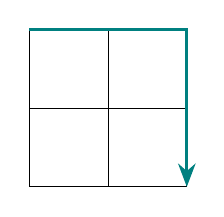
\begin{tikzpicture}
			\draw (0, 0) grid +(2,2);
			\draw[very thick, -Stealth, blue!50!green] (0, 2) -| (2, 0);
		\end{tikzpicture}
		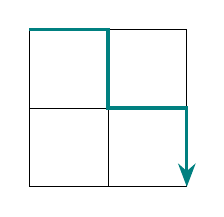
\begin{tikzpicture}
			\draw (0, 0) grid +(2,2);
			\draw[very thick, -Stealth, blue!50!green] (0, 2) -| (1, 1) -| (2,0);
		\end{tikzpicture}
		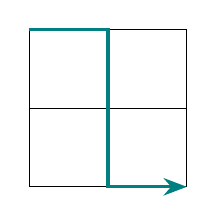
\begin{tikzpicture}
			\draw (0, 0) grid +(2,2);
			\draw[very thick, -Stealth, blue!50!green] (0, 2) -| (1, 0) -- (2, 0);
		\end{tikzpicture}

		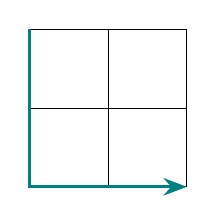
\begin{tikzpicture}
			\draw (0, 0) grid +(2,2);
			\draw[very thick, -Stealth, blue!50!green] (0, 2) |- (2, 0);
		\end{tikzpicture}
		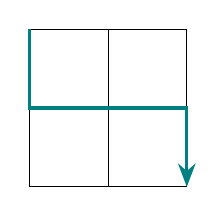
\begin{tikzpicture}
			\draw (0, 0) grid +(2,2);
			\draw[very thick, -Stealth, blue!50!green] (0, 2) |- (1, 1) -| (2,0);
		\end{tikzpicture}
		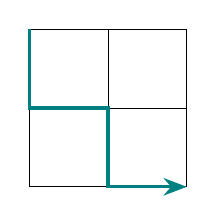
\begin{tikzpicture}
			\draw (0, 0) grid +(2,2);
			\draw[very thick, -Stealth, blue!50!green] (0, 2) |- (1, 1) |- (2,0);
		\end{tikzpicture}
	\end{center}

	在一个 $20 \times 20$ 的网格中,从左上角到右下角的路径,每次只能向右或向下移动一次。有多少条不同的路径从起点到终点?
\end{tcolorbox}

\subsection{算法}
这道题目要用到动态规划来解,最上边的第一个节点都依赖于其左边的节点有多少路径,与最上边相似,最左边的节点都依赖其上面的节点,在这里最上边与最左边的节点的路径数都为1。其他节点都依赖于其上方与左边的节点的数量,因此可以写成下面的伪代码:
\begin{algorithm}
	\caption{网格路径数}
	\begin{algorithmic}[1]
	\State 初始化一个 $(N+1) \times (N+1)$的矩阵,第1行全部为1,第一列也全部为1
	\State 遍历除第一行和第一列以外的节点,每个节点的值等于上方的值+左边的值
	\end{algorithmic}
\end{algorithm}


\subsection{答案}
137846528820

\section{数字的数字和}
\subsection{问题描述}
\begin{tcolorbox}
2 的 15 次方是 32768,其数字和为 3 + 2 + 7 + 6 + 8 = 26。

计算 2 的 1000 次方的数字和是多少?
\end{tcolorbox}

\subsection{算法}
可以将字符串数字类中实现一个乘法,在乘法的基础上实现幂运算。然后还需要实现一个计算数字和的函数。

\subsection{答案}

\section{数字文字计数}
\subsection{问题描述}
\begin{tcolorbox}
	如果将 1 到 5 写成英文单词,它们分别是:

	\begin{itemize}
		\forcsvlist{\item}{
		      1 = "one",
		      2 = "two",
		      3 = "three",
		      4 = "four",
		      5 = "five",
		      }
	\end{itemize}
	这些单词的字母数量为 3、3、5、4 和 4。因此,1 到 5 的数字单词一共有
	$ 3 + 3 + 5 + 4 + 4 = 19 $
	个字母。

	从 1 到 1000(含 1000)中的每个数字用英文单词来表示,不计空格和连字符,总共有多少个字母?

	例如:
	342(three hundred and forty-two)包含 23 个字母。

	115(one hundred and fifteen)包含 20 个字母。

	注意:不计空格或连字符,"and" 是按规则包含在使用中的英文单词中。
\end{tcolorbox}

\subsection{算法}
\begin{enumerate}
	\item 准备数字到英文单词的映射表:我们需要将 1 到 19 的单词直接映射。对于整十数(20, 30, ..., 90),也要单独映射。然后为“hundred”(100)和“thousand”(1000)定义规则。
	\item 分段处理数字:例如,对于 342,英文单词表示为 \textit{three hundred and forty-two}。我们可以将数字拆分为百位数、十位数、个位数,分别进行转换。
	\item 处理特殊情况:例如 100 到 999 之间的数字,需要注意添加 "and"。
	\item 统计字母数:统计所有数字转换成单词后的字母数量,不计空格和连字符。
\end{enumerate}

\subsection{答案}
21124

\section{最大路径和}
\subsection{问题描述}
\begin{tcolorbox}
	给定一个三角形,从顶部到底部选择一条路径,使得路径上的数字总和最大。如下所示:

	\[
		\begin{aligned}
			  &   &                    & \textcolor{red}{3} &                    &   &   \\
			  &   & \textcolor{red}{7} &                    & 4                  &   &   \\
			  & 2 &                    & \textcolor{red}{4} &                    & 6 &   \\
			8 &   & 5                  &                    & \textcolor{red}{9} &   & 3
		\end{aligned}
	\]

	在这个例子中,最大的路径和为 23。请找到这个最大路径和。

	\begin{center}
		75\\
		95 64\\
		17 47 82\\
		18 35 87 10\\
		20 04 82 47 65\\
		19 01 23 75 03 34\\
		88 02 77 73 07 63 67\\
		99 65 04 28 06 16 70 92\\
		41 41 26 56 83 40 80 70 33\\
		41 48 72 33 47 32 37 16 94 29\\
		53 71 44 65 25 43 91 52 97 51 14\\
		70 11 33 28 77 73 17 78 39 68 17 57\\
		91 71 52 38 17 14 91 43 58 50 27 29 48\\
		63 66 04 68 89 53 67 30 73 16 69 87 40 31\\
		04 62 98 27 23 09 70 98 73 93 38 53 60 04 23\\
	\end{center}
\end{tcolorbox}

\subsection{算法}
这道题目用动态规划的方法来求解。

\subsection{答案}
1074

\section{标题}
\subsection{问题描述}
\begin{tcolorbox}
在1901年1月1日到2000年12月31日的这段时间内,有多少个月的1号是星期天?已知:
\begin{itemize}
    \item 1900年1月1日是星期一;
    \item 闰年规则为:如果年份能被4整除但不能被100整除,或者能被400整除,则该年为闰年;
    \item 每月天数:
    \begin{itemize}
        \item 31天:1月、3月、5月、7月、8月、10月、12月;
        \item 30天:4月、6月、9月、11月;
        \item 28天:2月,闰年为29天。
    \end{itemize}
\end{itemize}
\end{tcolorbox}

\subsection{算法}
先实现一个闰年判断的函数
\begin{algorithm}
	\caption{算法标题}
	\begin{algorithmic}[1]
		\If{$Y \mod 400 = 0$ or $(Y \mod 4 = 0$ and $Y \mod 100 \neq 0) $}
		\Return \textbf{true}
	\EndIf
	\end{algorithmic}
\end{algorithm}

\subsection{答案}

\section{阶乘数字和}
\subsection{问题描述}
\begin{tcolorbox}
求 $100!$ 的各位数字和。即:
\[
100! = 100 \times 99 \times \cdots \times 2 \times 1
\]
计算得到的阶乘结果后,求其各位数字的和。例如:
\[
10! = 10 \times 9 \times \cdots \times 1 = 3628800
\]
其各位数字之和为:
\[
3 + 6 + 2 + 8 + 8 + 0 + 0 = 27
\]
\end{tcolorbox}

\subsection{算法}
用前面实现的字符串数字类中添加个阶乘的算法。

\subsection{答案}
648

\section{亲和数之和}\label{sec:problem21}
\subsection{问题描述}
\begin{tcolorbox}
	定义 $d(n)$ 表示 $n$ 的所有真因数(即小于 $n$ 的除 $n$ 之外的除数)的和。

	如果 $d(a) = b$ 且 $d(b) = a$,并且 $a \neq b$,那么 $a$ 和 $b$ 被称为亲和数。例如,220 和 284 就是一对亲和数:

	\[
		d(220) = 1 + 2 + 4 + 5 + 10 + 11 + 20 + 22 + 44 + 55 + 110 = 284
	\]
	\[
		d(284) = 1 + 2 + 4 + 71 + 142 = 220
	\]

	求小于10000的所有亲和数的和。
\end{tcolorbox}

\subsection{算法}
\begin{enumerate}
	\item 编写函数 $d(n)$,计算 $n$ 的所有真因数的和。
	\item 对于每个小于10000的数字 $a$,计算 $b = d(a)$,如果 $d(b) = a$ 且 $a \neq b$,则 $a$ 和 $b$ 是亲和数。
	\item 注意避免重复计算。
\end{enumerate}

\subsection{答案}
31626

\section{名字记分}\label{sec:problem22}
\subsection{问题描述}
\begin{tcolorbox}

给定一个超过五千个名字的文件,将这些名字按字母顺序排序。然后,对于每个名字,按以下步骤计算得分:

\begin{enumerate}
    \item 计算名字的字母值:将名字中每个字母的字母顺序($A=1, B=2, ..., Z=26$)相加。例如,$COLIN$ 的字母值为 $3 + 15 + 12 + 9 + 14 = 53$。
    \item 将名字的字母值乘以其在排序后的位置索引,得到名字的得分。例如,"COLIN" 在排序后是第938个名字,其得分为 $938 \times 53 = 49714$。
\end{enumerate}
\end{tcolorbox}

\subsection{算法}
\begin{enumerate}
    \item 读取文件并去除名字的引号。
    \item 按字母顺序对名字进行排序。
    \item 对于每个名字,计算其字母值,并乘以其在排序中的位置,计算名字得分。
    \item 将所有名字的得分相加,得到结果。
\end{enumerate}

\subsection{答案}
871198282

\section{非盈数之和}\label{sec:problem23}
\subsection{问题描述}
\begin{tcolorbox}
	如果一个数的真因数之和大于该数本身,则称该数为\textbf{盈数}。例如,$12$ 是最小的盈数,它的真因数之和为:
	\[
		1 + 2 + 3 + 4 + 6 = 16
	\]
	大于12。找出所有不能写成两个盈数之和的正整数,并求它们的总和。

	已知:所有大于28123的数字都可以写成两个盈数之和,因此我们只需考虑小于等于28123的数字。

\end{tcolorbox}

\subsection{算法}
\begin{enumerate}
	\item \textbf{判断盈数}:编写函数判断某个数是否为盈数。
	\item \textbf{生成盈数}:找出所有小于等于28123的盈数。
	\item \textbf{判断是否为两个盈数之和}:通过分解一个数字为两个部分,分别计算是否为盈数。
	\item \textbf{求和}:遍历所有小于等于28123的数字,计算那些不能表示为两个盈数之和的数字总和。
\end{enumerate}

\subsection{答案}
4179871

\section{标题}
\subsection{问题描述}
\begin{tcolorbox}
排列是对象的一种有序排列。例如,3124 是数字 1、2、3 和 4 的一种可能的排列。如果所有排列都按数值或字母顺序列出,我们称之为字典序。数字 0、1 和 2 的字典序排列如下:

\begin{enumerate}
  \item 012
  \item 021
  \item 102
  \item 120
  \item 201
  \item 210
\end{enumerate}

请问数字 0、1、2、3、4、5、6、7、8 和 9 的第 1,000,000 个字典序排列是什么?
\end{tcolorbox}

\subsection{算法}
排列的算法是从数组的最右边开始搜索,如果打到一个元素,其左边(P)的值比自身小,再从左到右搜索一个比P大的值,则两个元素对调,然后对P右边的元素从小到大排序。

\subsection{答案}
2783915604

\section{第一个有1000位数的斐波那契数}
\subsection{问题描述}
\begin{tcolorbox}

斐波那契数列定义为:

\[
F_1 = 1, \quad F_2 = 1, \quad F_n = F_{n-1} + F_{n-2} \, \text{对} \, n \geq 3.
\]

求第一个有1000位的斐波那契数 \( F_n \) 的序号。
\end{tcolorbox}

\subsection{算法}
用之前实现的字符串数字类可以轻松解决这个问题。

\subsection{答案}
4782

\section{倒数的循环节}\label{sec:problem26}
\subsection{问题描述}
\begin{tcolorbox}
单位分数指的是分子为 1 的分数。分母为 2 到 10 的所有单位分数的小数部分如下所示:

\[
\frac{1}{2} = 0.5
\]
\[
\frac{1}{3} = 0.\overline{3}
\]
\[
\frac{1}{4} = 0.25
\]
\[
\frac{1}{5} = 0.2
\]
\[
\frac{1}{6} = 0.1\overline{6}
\]
\[
\frac{1}{7} = 0.\overline{142857}
\]
\[
\frac{1}{8} = 0.125
\]
\[
\frac{1}{9} = 0.\overline{1}
\]
\[
\frac{1}{10} = 0.1
\]

可以看出,\( \frac{1}{7} \) 有一个 6 位的循环节。

找出小于 1000 的所有单位分数中,小数部分循环节最长的分数的分母。
\end{tcolorbox}

\subsection{算法}
当分子小于分母的时候乘以10直到大于分母为止。

分子与分母求余,并将余数记录下来,如果出现相同的余数则视为循环出现。

\subsection{答案}

\section{二次表达式生成的素数}
\subsection{问题描述}
\begin{tcolorbox}
欧拉发现了这个著名的二次表达式:

\[
n^2 + n + 41
\]

对于 \( n = 0 \) 到 \( n = 39 \) 之间的每个 \( n \),该表达式生成了 40 个素数。然而,当 \( n = 40 \) 时,得到的 \( 40^2 + 40 + 41 = 1681 \) 并不是一个素数。该二次表达式生成了从 \( n = 0 \) 到 \( n = 39 \) 的连续素数。

发现了以下的二次表达式:

\[
n^2 - 79n + 1601
\]

对于 \( n = 0 \) 到 \( n = 79 \) 之间的每个 \( n \),该表达式生成了 80 个素数。这一表达式生成的连续素数的系数积为 \( -79 \) 和 1601,积为 \( -79 \times 1601 = -126479 \)。

考虑形如 \( n^2 + an + b \) 的二次表达式,其中 \( |a| < 1000 \) 且 \( |b| \leq 1000 \)。

找出系数 \( a \) 和 \( b \) 使得表达式 \( n^2 + an + b \) 对于从 \( n = 0 \) 开始的连续整数 \( n \) 生成最多的素数,计算出此时 \( a \) 和 \( b \) 的乘积。

\end{tcolorbox}

\subsection{算法}
最简单粗暴的方法是直接两遍循环,但是这种方法的消耗是指数级增长的。我们可以对暴力循环进行一些优化。

\begin{itemize}
  \item 首先,我们来考虑 \( b \),当 \( n = 0 \),二项式的值为 \( b \),所以 \( b \)必须为素数才行;
  \item \( a \)的值比较自由,但是也有可以考虑的点,比如当 \( n = 1 \)时,二项式的值为 \( 1 + a + b
    \),除了值等于2的情况,其他情况下, \( a \)和 \( b \)的奇偶性必须是相同的。
\end{itemize}

\subsection{答案}

\section{螺旋矩阵对角线之和}
\subsection{问题描述}
\begin{tcolorbox}

	从数字1开始,按顺时针顺序依次将连续的奇数排列成一个边长为 5 的螺旋矩阵如下所示:

	\[
		\begin{matrix}
			\red{21} & 22      & 23      & 24      & \red{25} \\
			20       & \red{7} & 8       & \red{9} & 10       \\
			19       & 6       & \red{1} & 2       & 11       \\
			18       & \red{5} & 4       & \red{3} & 12       \\
			\red{17} & 16      & 15      & 14      & \red{13}
		\end{matrix}
	\]

	可以看到,该矩阵对角线上的数字之和为 101。

	考虑更大的边长为 1001 的螺旋矩阵,求该矩阵对角线上的数字之和。
\end{tcolorbox}

\subsection{算法}
对角线数字的生成方法为:
\begin{itemize}
	\item 从1开始,第二层矩阵的对角线四个角点分别加2;
	\item 下一层的矩阵的步长要加2;
\end{itemize}

\subsection{答案}
669171001

\section{不同幂次之和}\label{sec:problem29}
\subsection{问题描述}
\begin{tcolorbox}
考虑所有形如 \( a^b \) 的幂次组合,其中 \( 2 \leq a \leq 5 \) 且 \( 2 \leq b \leq 5 \):

\[
2^2 = 4, \quad 2^3 = 8, \quad 2^4 = 16, \quad 2^5 = 32
\]
\[
3^2 = 9, \quad 3^3 = 27, \quad 3^4 = 81, \quad 3^5 = 243
\]
\[
4^2 = 16, \quad 4^3 = 64, \quad 4^4 = 256, \quad 4^5 = 1024
\]
\[
5^2 = 25, \quad 5^3 = 125, \quad 5^4 = 625, \quad 5^5 = 3125
\]

如果将这些幂次组合按大小排列并去除重复的项,我们得到如下的序列:

\[
4, 8, 9, 16, 25, 27, 32, 64, 81, 125, 243, 256, 625, 1024, 3125
\]

这些组合一共有 15 项。

考虑所有形如 \( a^b \) 的幂次组合,其中 \( 2 \leq a \leq 100 \) 且 \( 2 \leq b \leq 100 \),求出这些幂次组合中不同的项有多少个。

\end{tcolorbox}

\subsection{算法}
这个问题的最主要问题是大数的处理,有了之前的字符串数字,解决这个问题就容易多了。

\subsection{答案}
9183

\section{数字的第五次幂}\label{sec:problem30}
\subsection{问题描述}
\begin{tcolorbox}

令人惊讶的是,只有三个数字可以写成它们各位数字的第四次幂之和:

\[
1634 = 1^4 + 6^4 + 3^4 + 4^4
\]

\[
8208 = 8^4 + 2^4 + 0^4 + 8^4
\]

\[
9474 = 9^4 + 4^4 + 7^4 + 4^4
\]

由于 $1 = 1^4$ 不是一个和,所以不包括在内。

这些数字的和是:

\[
1634 + 8208 + 9474 = 19316
\]

找出所有可以写成它们各位数字的第五次幂之和的数字的总和。
\end{tcolorbox}

\subsection{算法}
这道题实现起来并不难,主要是考虑判断的边界问题,这里的判断是到6位数为止,因为6位数最大为\num{999999},其数字的5次方之和为\num{354294},已经小于\num{999999}。而如果增加到7位数,最小的7位数是\num{1000000},而即使是\num{9999999}的数字5次方之和也只有\num{413343}。

另外一个可以优化的地方是可以将0--9所有数字的5次方计算出来,后面直接从数组中读取可以避免重复计算的问题。

\subsection{答案}
443839

\section{硬币组合}
\subsection{问题描述}
\begin{tcolorbox}

	在英国,硬币有1p、2p、5p、10p、20p、50p、£1 和 £2 的面额。计算有多少种不同的方式可以用这些硬币组合成总额为 £2?
\end{tcolorbox}

\subsection{算法}
这种问题用动态规划解决是最佳方案。用一个数组\texttt{dp}来记录每增加一种硬币方案数量的变化。

主要实现思路如下:
\begin{enumerate}
	\item 初始化一个 \( 200 + 1 \)长度的 \( dp \)数组, \( dp[0] = 1 \);
	\item 遍历所有币种,每种币种从其币值 \( m \)开始 \( dp[x] += dp[x - m] \)
\end{enumerate}

\subsection{答案}
73682

\section{标题}
\subsection{问题描述}
\begin{tcolorbox}
	我们称一个 $n$ 位数字为“全数字”的,如果它恰好使用了从 1 到 $n$ 的所有数字一次;例如,5 位数字 $15234$ 就是 1 到 5 的全数字。

	数字 $7254$ 是不寻常的,因为等式 $39 \times 186 = 7254$ 中的乘数、乘数和乘积都是 1 到 9 的全数字。

	找出所有乘数/乘数/乘积等式可以写成 1 到 9 的全数字的所有乘积的和。

	提示:有些乘积可以通过不止一种方式获得,因此确保在你的总和中只包含一次。
\end{tcolorbox}

\subsection{算法}

\subsection{答案}
$45228$

\section{数字抵消分数}
\subsection{问题描述}
\begin{tcolorbox}
	分数 \( \frac{49}{98} \) 是一个有趣的分数,因为一个没有经验的数学家在尝试简化它时可能会错误地认为 \( \frac{49}{98} = \frac{4}{8} \),这是正确的,是通过取消数字 9 得到的。

	我们将考虑像 \( \frac{30}{50} = \frac{3}{5} \) 这样的分数作为平凡的例子。

	在数值小于1且分子分母都包含两位数的分数中,恰好有四个非平凡的例子。

	如果这四个分数的乘积以最简形式给出,求分母的值。
\end{tcolorbox}

\subsection{算法}
根据要求分子必须比分母小,所以经过简单的推算,可以抵消的必须要错位,就是抵消分子的10位数的话,分母上就需要是个位。

假设 \( \frac{ax}{bx} = \frac{a}{b} \), 则有 \(  (10a + x) b = (10b + x) a \),进一步化简可以得到 \( a = b
\),这样分子就等于分母,与题目中分数的值要小于1不符。同样也可以证明不能是分子分母的10位相同。

\subsection{答案}
\( 100 \)

\section{标题}
\subsection{问题描述}
\begin{tcolorbox}

	由于 $1! + 2! + 145! = 145$,因此,145 是一个特殊的数。请找出所有满足以下条件的数的和:
	\begin{itemize}
		\item 这些数等于它们各个数字阶乘的和。
	\end{itemize}

	\textbf{数学公式}:

	一个数 $n$ 被称为特殊数,如果
	\[
		n = \sum_{i=1}^{k} d_i!
	\]
	其中 $d_i$ 是 $n$ 的每一位数字,$k$ 是数字的位数。
\end{tcolorbox}

\subsection{算法}
在最开始的时候数字的阶乘和增长很快, \( 9! = 362880
\),但是数字随着位数的增长速度变得更快,\num{999999}的数字阶乘和为\num{2177280},\num{9999999}为\num{2540160},后面数字位数增长引发值增大的速度远远超过了数字阶乘和,所以只需要判断到7位数就OK了。

\subsection{答案}

\section{环形素数}
\subsection{问题描述}
\begin{tcolorbox}

素数 \( p \) 称为环形素数,如果其所有旋转都是素数。例如,13 是一个环形素数,因为它的旋转 13 和 31 都是素数。

考虑所有小于 1,000,000 的环形素数的总数。
\end{tcolorbox}

\subsection{算法}
这道题只需要解决如何构造环形数的问题即可,结合之前的素数判断的方法即可解决此问题。

构造环形数只需要计算出数$n$的位数$p$,将数 \( n \)分成两部分, \( p - 1 \)位 \( b \)和最后一个数字 \( e \),新的生成数即为:
\begin{equation*}
 10^pe + b
\end{equation*}
将这个过程循环 \( p \)次即可完成变化。


\subsection{答案}
55

\section{十进制和二进制回文数}\label{sec:problem36}
\subsection{问题描述}
\begin{tcolorbox}

回文数是左到右和从右到左读起来都一样的数。例如,585 是一个回文数。

在十进制和二进制表示下,某些回文数同时也是回文数。例如,585 是一个回文数(十进制),在二进制表示下也是一个回文数:1001001001。

找到所有小于 1,000,000 的数字中,既是十进制回文数又是二进制回文数的数字之和。
\end{tcolorbox}

\subsection{算法}
回文数的判定之前已经写过,所以只需要实现二进制回文数的判定,这个可以用回文数判定的算法,将基数变为2即可。


\subsection{答案}
872187

\section{可截素数}\label{sec:problem37}
\subsection{问题描述}
\begin{tcolorbox}

可截素数指的是:从左到右和从右到左逐位截去数字后,剩下的所有数字仍然是素数。例如,3797 是一个可截素数:

\begin{itemize}
    \item 从左到右依次截去:3797、797、97、7 都是素数;
    \item 从右到左依次截去:3797、379、37、3 也是素数。
\end{itemize}

只考虑两位数及以上的素数,求所有这样的素数之和(一共只有11个)。

\end{tcolorbox}

\subsection{算法}

依次用 \( 10, 100, \cdots \) 来对要判断的质数 \( n \)取余,并依次判断余数是不是质数。

\subsection{答案}
748317

\section{全数字乘积}\label{sec:problem38}
\subsection{问题描述}
\begin{tcolorbox}

将 192 与 1、2 和 3 分别相乘:

\[
192 \times 1 = 192
\]
\[
192 \times 2 = 384
\]
\[
192 \times 3 = 576
\]

将这些乘积连接起来,我们得到一个 1 到 9 的全数字(192384576)。我们称 192384576 为 192 和 (1,2,3) 的连接乘积。

同样,对于 9 和 (1,2,3,4,5),我们可以得到全数字 918273645,这是一个 1 到 9 的全数字。

所求是能通过某个整数和 (1,2,...) 的倍数产生的最大全数字 1 到 9 的连接乘积。该整数不能有重复的数字,且必须包含每个数字恰好一次。
\end{tcolorbox}

\subsection{算法}
对于每一个 \( 123456789 \)的排列,测试以下几种情况:
\begin{enumerate}
	\item 将第1位数依次乘以23456789
	\item 取前面2位数
	\item 取前面3位数
	\item 取前面4位数
\end{enumerate}
5位数不用再考查,因为加起来会超过10位数。

因为是求最大的连接乘积,所以可以从最大的987654321开始用prev\_permutation函数。

\subsection{答案}
932718654

\section{整数边长直角三角形}
\subsection{问题描述}
\begin{tcolorbox}

	如果一个直角三角形的边长为整数,则其周长 \( p \) 是边长的和。对于周长 \( p = 120 \),有三个不同的解:

	\[
		(20, 48, 52),\ (24, 45, 51),\ (30, 40, 50)
	\]

	对于给定的 \( p \leq 1000 \),找出具有最多解的 \( p \) 值。
\end{tcolorbox}

\subsection{算法}
斜边小于两个直角边之和。

\subsection{答案}

\section{Champernowne 常数}
\subsection{问题描述}
\begin{tcolorbox}

	Champernowne 常数是通过将正整数序列连接起来构成的一个无限小数。例如:

	\[
		0.123456789101112131415161718192021\ldots
	\]

	这个小数包含了所有的正整数数字,依次排列。

	给定 Champernowne 常数的第 \( n \) 位是指小数中第 \( n \) 位的数字。

	求出下列位置上的数字的乘积:

	\[
		d_1 \times d_{10} \times d_{100} \times d_{1000} \times d_{10000} \times d_{100000} \times d_{1000000}
	\]

	其中 \( d_n \) 表示 Champernowne 常数中第 \( n \) 位的数字。
\end{tcolorbox}

\subsection{算法}
\begin{enumerate}
	\item 将$ n $ 循环减去 \( 9, 90 \times 2, 900 \times 3 \)直到 \( n \) 小于当前数字宽带的数字的总和。
	\item 将 \( n \) 与当前的数字宽度求余,再加之前的所有数字即得到第 \( n \)位数对应的数 \( P \)
	\item 将 \( P \) 与当前数字宽度求余即可取出相应的数字
\end{enumerate}

\subsection{答案}

\section{全数字素}\label{sec:problem41}
\subsection{问题描述}
\begin{tcolorbox}
一个 $n$ 位全数字数是指包含数字 $1$ 到 $n$ 中所有数字的排列且没有重复的数。例如,$2143$ 是一个 4 位全数字数,并且它恰好是一个素数。

求最大的全数字素数。
\end{tcolorbox}

\subsection{算法}
9位数和8位数的全数字之和分别是45和36,均是3的倍数,所以不可能是素数。可以从7654321开始,判断是不是素数,如果不是,再用perv\_permutation来生成一个排列,直到找到目标为止。

\subsection{答案}
7652413

\section{编码三角形数}
\subsection{问题描述}
\begin{tcolorbox}
	三角形数的生成公式为 $T_n = \frac{n(n+1)}{2}$,它的前十项是:

	\begin{equation*}
		1 , 3 , 6 , 10 , 15 , 21 , 28 , 36 , 45 , 55 , \cdots
	\end{equation*}
	给定一个单词的字母值,假设 $A=1, B=2, ..., Z=26$,则单词的字母值为所有字母对应数值的和。例如,单词 "SKY" 的字母值为
	$19 + 11 + 25 = 55$,它恰好是一个三角形数。

	在提供的\href{https://projecteuler.net/resources/documents/0042_words.txt}{文本文件}中包含了一系列单词,计算出其中有多少个单词的字母值是三角形数。
\end{tcolorbox}
\subsection{算法}
\begin{enumerate}
	\item 读取文件中的名字到数组
	\item 根据名字最大长度并假设每个字母都是 $Z$,计算出最大的分数
	\item 用三角形数公式生成能够覆盖最大名字分数的所有三角形数
	\item 用每个名字的分法在生成的三角形数中查找
\end{enumerate}

\subsection{答案}
162

\section{全数字的部分整除性}
\subsection{问题描述}
\begin{tcolorbox}
将0到9这十个数字以某种排列组合的形式组成一个10位数,称为全数字数。例如,1406357289 是一个全数字数。

假设 \( d_1 \) 表示第一个数字,\( d_2 \) 表示第二个数字,依此类推。我们定义如下特性:

\begin{itemize}
	\item \( d_2d_3d_4 \) 能被 2 整除
	\item \( d_3d_4d_5 \) 能被 3 整除
	\item \( d_4d_5d_6 \) 能被 5 整除
	\item \( d_5d_6d_7 \) 能被 7 整除
	\item \( d_6d_7d_8 \) 能被 11 整除
	\item \( d_7d_8d_9 \) 能被 13 整除
	\item \( d_8d_9d_{10} \) 能被 17 整除
\end{itemize}

找到所有满足上述特性的全数字数,并求它们的和。

\end{tcolorbox}

\subsection{算法}
用 \( 0123456789 \)的排列变化来逐项进行判断,但是因为0不能放在首位,所以可以从 \( 1023456789 \)开始。

还有一个可以优化的地方,因为\texttt{next\_permutation}是从最右边开始变化的,所以可以先从右边开始判断。

\subsection{答案}

\section{五边形数}
\subsection{问题描述}
\begin{tcolorbox}
	五边形数由公式 $P_n = \dfrac{n(3n-1)}{2}$ 给出。前十个五边形数是:

	\[
		1, 5, 12, 22, 35, 51, 70, 92, 117, 145, \dots
	\]

	可以看出,$P_4 + P_7 = 22 + 70 = 92 = P_8$,但是它们的差 $70 - 22 = 48$ 不是五边形数。

	找出满足条件的五边形数对 $P_j$ 和 $P_k$,使得它们的和与差均为五边形数,并且 $D = |P_k - P_j|$ 的值最小。
\end{tcolorbox}

\subsection{算法}


\subsection{答案}

\section{复合多边形数}
\subsection{问题描述}
\begin{tcolorbox}
	三角形数、五边形数和六边形数由以下公式给出:

	\[
		T_n = \frac{n(n + 1)}{2}
	\]
	\[
		P_n = \frac{n(3n - 1)}{2}
	\]
	\[
		H_n = n(2n - 1)
	\]

	可以发现,285 是一个三角形数、五边形数、也是一个六边形数,且对应的值是 40755。

	找出下一个既是三角形数、五边形数、也是六边形数的数。

\end{tcolorbox}

\subsection{算法}

\subsection{答案}

\section{哥德巴赫的其他猜想}
\subsection{问题描述}
\begin{tcolorbox}
克里斯蒂安·哥德巴赫曾经提出了一个猜想:任何一个大于2的奇合数都可以写成一个素数加上一个平方数的两倍,即:

\[
n = p + 2 \times k^2
\]

其中,\( n \) 是奇合数,\( p \) 是素数,\( k \) 是一个正整数。

这个猜想后来被证明是错误的。也就是说,存在一个奇合数无法用上述方式表示。

找出最小的那个不能被写成素数加上两倍平方数的奇合数。
\end{tcolorbox}

\subsection{算法}
可以生成一个素数表,将奇合数依次减去各个素数,然后判断差的一半是不是个平方数。

\subsection{答案}
5777

\section{不同质因数}\label{sec:problem47}
\subsection{问题描述}
\begin{tcolorbox}
找出第一个有四个不同质因数的连续整数。换句话说,每个数都有恰好四个不同的素因数。 

例如,第一个有两个不同质因数的连续整数是:

\[
14 = 2 \times 7
\]
\[
15 = 3 \times 5
\]

现在,找出第一个有四个不同质因数的连续四个整数。

\end{tcolorbox}

\subsection{算法}
生成一个素数表,计算数字有多少个不同的质因数,如果连续4个数的质因数都是4个,就找到答案。


\subsection{答案}
134043

\section{标题}
\subsection{自幂之和}
\begin{tcolorbox}

计算以下表达式的最后十位数:

\[
1^1 + 2^2 + 3^3 + \cdots + 1000^{1000}
\]


\end{tcolorbox}

\subsection{算法}
这又是一道大整数计算的题目,用之前实现的bigint可以轻松解决。


\subsection{答案}
9110846700

\section{素数排列}
\subsection{问题描述}
\begin{tcolorbox}
考虑由三个不同的素数组成的等差数列,这三个素数由相同的数字重排组成。比如,1487、4817 和 8147 就是这样的一个序列。

这个序列有一个显著的性质:1487、4817 和 8147 是三个 4 位数,并且每一个都是素数。更有趣的是,这三个数字的差值相同:4817 - 1487 = 3330,8147 - 4817 = 3330。

还有一个 4 位数的递增序列也满足这个性质,但它并不是将 1487、4817 和 8147 简单重排所得。找到这个序列,并将其三个项连接起来形成 12 位数。这个 12 位数是多少?
\end{tcolorbox}

\subsection{算法}
生成1万以内的素数数组,从1000开始验证,如果是素数的情况下,再进行一次内循环,检查数字是否为素数,与外循环的数是否数字相同。然后计算出第三个数,需要满足的条件的是第三个数要小于10000,并且是素数,而且与外循环或者内循环的数字相同。

\subsection{答案}
296962999629

\section{连续素数和}
\subsection{问题描述}
\begin{tcolorbox}
	素数41可以写成6个连续素数之和:

	\[
		41 = 2 + 3 + 5 + 7 + 11 + 13
	\]

	这也是一个素数。

	同样地,100以下最长的连续素数和是953,由21个连续素数相加得到:
	\begin{multline*}
		953 = 7 + 11 + 13 + 17 + 19 + 23 + 29 + 31 + 37 + 41 + 43 + 47 + 53 + 59 + 61\\ + 67 + 71 + 73 + 79 + 83
	\end{multline*}

	找出小于一百万的素数中,可以写成连续素数和的最长序列的素数。

\end{tcolorbox}

\subsection{算法}
用欧拉筛生成素数数组,从2开始连续加,找到不超过1百万的最大长度,如果在这个长度找不到,就长度减一,就这样循环搜索,直到找到答案。

\subsection{答案}
997651

\section{素数数字替换}
\subsection{问题描述}
\begin{tcolorbox}
	通过将素数中的某些(不一定连续的重复数字)位替换成相同的数字,可以生成一个素数家族。例如,位于56003的第三位和第四位替换成相同的数字,我们可以得到以下十个数:

	\[
		56003, 56113, 56223, 56333, 56443, 56553, 56663, 56773, 56883, 56993
	\]

	其中,满足素数条件的有7个:56003, 56113, 56333, 56443, 56663, 56773 和 56993。

	在这些素数中,56003是第一个在这种情况下可以产生一个七素数家族的成员。

	找出满足这个性质的八素数家族的最小素数。
\end{tcolorbox}

\subsection{算法}
\begin{enumerate}
	\item 用埃氏筛法筛出素数
	\item 将素数转换为字符串
	\item 对字符串按数字查找,如果找到重复的数字则进行替换并判断替换后的数字是否为素数,如果找个8个就退出
\end{enumerate}

\subsection{答案}

\section{排列倍数}
\subsection{问题描述}
\begin{tcolorbox}
	可以看出,数字 125874 与其两倍 251748 含有完全相同的数字,但顺序不同。

	找出最小的正整数 $x$,使得 $2x, 3x, 4x, 5x, 6x$ 含有完全相同的数字。
\end{tcolorbox}

\subsection{算法}
只要实现是一个判断相同数字的算法即可解决这个问题。

\begin{enumerate}
	\item 将数字分别转换成字符串
	\item 将字符串排序
	\item 比较两个字符串
\end{enumerate}

\subsection{答案}
142857

\section{组合数计算}\label{sec:problem53}
\subsection{问题描述}
\begin{tcolorbox}
已知有 10 种从 5 个数 12345 中选出 3 个数的方法:

\[ 
123, 124, 125, 134, 135, 145, 234, 235, 245, 345 
\]

在组合数学中,我们使用以下符号来表示组合数:

\[
\binom{5}{3} = 10
\]

一般来说,组合数公式为:

\[
\binom{n}{r} = \frac{n!}{r!(n - r)!}
\]

其中,\(r \leq n\),且 \(n! = n \times (n-1) \times \cdots \times 1\),且 \(0! = 1\)。

当 \(n = 23\) 时,组合数首次超过 100 万:

\[
\binom{23}{10} = 1144066
\]

问题:在 \( 1 \leq n \leq 100 \) 的范围内,有多少个不一定互不相同的组合数 \( \binom{n}{r} \) 的值大于一百万?

\end{tcolorbox}

\subsection{算法}
这道题当然可以用设计的大数来解决,但是如果采取一些优化算法还是可以避免溢出的。

分子与分母每一次计算时都用最小公倍数来减小。

第二种是用combination的另外一个递推公式:
\begin{equation*}
\binom{n}{r}=\binom{n-1}{r-1}+\binom{n-1}{r}
\end{equation*}
这个方法更高效和通用,也不会有溢出的风险。
\subsection{答案}
4075

\section{Poker hands}
Problem 54

In the card game poker, a hand consists of five cards and are ranked, from lowest to highest, in the following way:

\rowcolors{0}{green!5}{white}
\noindent
\begin{tablebox}{\textsc{Poker Hands}}
	{
		\color{black!70} \sffamily
		\begin{tabularx}{\textwidth}{rX}
			High Card       & Highest value card                            \\
			One Pair        & Two cards of the same value                   \\
			Two Pairs       & Two different pairs                           \\
			Three of a Kind & Three cards of the same value                 \\
			Straight        & All cards are consecutive values              \\
			Flush           & All cards of the same suit                    \\
			Full House      & Three of a kind and a pair                    \\
			Four of a Kind  & Four cards of the same value                  \\
			Straight Flush  & All cards are consecutive values of same suit \\
			Royal Flush     & Ten, Jack, Queen, King, Ace, in same suit     \\
		\end{tabularx}
	}
\end{tablebox}

The cards are valued in the order:
2, 3, 4, 5, 6, 7, 8, 9, 10, Jack, Queen, King, Ace.

If two players have the same ranked hands then the rank made up of the highest value wins; for example, a pair of eights
beats a pair of fives (see example 1 below). But if two ranks tie, for example, both players have a pair of queens, then
highest cards in each hand are compared (see example 4 below); if the highest cards tie then the next highest cards are
compared, and so on.

Consider the following five hands dealt to two players:

\begin{tablebox}{\textsc{Examples}}
	\color{black!70} \sffamily
	\begin{tabularx}{\textwidth}{c X X c}
		{\textbf{Hand}} & {\textbf{Player 1}}                                             & {\textbf{Player 2}}                                              & {\textbf{Winner}} \\
		1               & 5H 5C 6S 7S KD \newline Pair of Fives                           & 2C 3S 8S 8D TD   \newline Pair of Eights                         & {Player 2}        \\
		2               & 5D 8C 9S JS AC\newline Highest card Ace                         & 2C 5C 7D 8S QH\newline Highest card Queen                        & {Player 1}        \\
		3               & 2D 9C AS AH AC\newline Three Aces                               & 3D 6D 7D TD QD\newline Flush with Diamonds                       & {Player 2}        \\
		4               & 4D 6S 9H QH QC\newline Pair of Queens\newline Highest card Nine & 3D 6D 7H QD QS\newline Pair of Queens\newline Highest card Seven & {Player 1}        \\
		5               & 2H 2D 4C 4D 4S\newline Full House With Three Fours              & 3C 3D 3S 9S 9D\newline Full House with Three Threes              & {Player 1}
	\end{tabularx}
\end{tablebox}
The file, poker.txt, contains one-thousand random hands dealt to two players. Each line of the file contains ten cards (separated by a single space): the first five are Player 1's cards and the last five are Player 2's cards. You can assume that all hands are valid (no invalid characters or repeated cards), each player's hand is in no specific order, and in each hand there is a clear winner.

How many hands does Player 1 win?

\rowcolors{0}{}{}

\section{Lychrel Numbers}

\subsection{Problem Description}
If we take \( 47 \), reverse and add,\( 47 + 74 = 121 \), which is palindromic.

Not all numbers produce palindromes so quickly. For example,
\begin{align*}
	349 + 943   & = 1292 \\
	1292 + 2921 & = 4213 \\
	4213 + 3124 & = 7337
\end{align*}

That is, \( 349 \) took three iterations to arrive at a palindrome.

Although no one has proved it yet, it is thought that some numbers, like \( 196 \)
, never produce a palindrome. A number that never forms a palindrome through the reverse and add process is called a
Lychrel number. Due to the theoretical nature of these numbers, and for the purpose of this problem, we shall assume
that a number is Lychrel until proven otherwise. In addition you are given that for every number below ten-thousand, it
will either (i) become a palindrome in less than fifty iterations, or, (ii) no one, with all the computing power that
exists, has managed so far to map it to a palindrome. In fact, \( 10677 \)
is the first number to be shown to require over fifty iterations before producing a palindrome:4668731596684224866951378664
(\( 53 \) iterations, \( 28 \) digits).

Surprisingly, there are palindromic numbers that are themselves Lychrel numbers; the first example is \( 4994 \).

How many Lychrel numbers are there below ten-thousand?

NOTE: Wording was modified slightly on 24 April 2007 to emphasise the theoretical nature of Lychrel numbers.

\subsection{Flow Chart}

\begin{tikzpicture}[node distance=2cm]
	\node [startstop] (start) {开始};
	\node [io, right of=start, xshift=4cm, text width=4cm] (io1) {输入一个考察的上限\\ 这里是10000};
	\node [operation, text width=2cm, below of=io1] (op1) {count = 0;\\ i = 10;};
	\node [decision, below of=op1, text width=2cm, yshift=-1cm] (dec1) {\( i < 上限 \)};
	\node [decision, below of=dec1, text width=2cm, yshift=-2cm] (dec2) {\( i \) is lychrel number?};
	\node [operation, below of=dec2, yshift=-1cm] (op2) {++count};
	\node [operation, right of=dec2, xshift= 4cm] (op3) {++i};
	\node [io, below of=op2] (io2) {输出count};
	\node [startstop, right of=io2, xshift=4cm] (stop) {结束};

	\draw[arrow] (start) -- (io1);
	\draw[arrow] (io1) -- (op1);
	\draw[arrow] (op1) -- (dec1);
	\draw[arrow] (dec1) -- node[right]{yes} (dec2);
	\draw[arrow] (dec1) -| node[right=.5cm, below=4cm]{no}([xshift=-2cm]io2.west) -- (io2);
	\draw[arrow] (dec2) -- node[right]{yes} (op2);
	\draw[arrow] (dec2) -- node[above]{no}(op3);
	\draw[arrow] (op3) |- (dec1);
	\draw[arrow] (io2) -- (stop);
\end{tikzpicture}

\chapter{Powerful Digit Sum}
\section{Description}
A googol ($10^{100}$) is a massive number: one followed by one-hundred zeros;
$100^{100}$is almost unimaginably large: one followed by two-hundred zeros. Despite their size, the sum of the digits in
each number is only .

Considering natural numbers of the form, $a^b$, where $a, b < 100$ what is the maximum digital sum?

\section{方根的渐进分数}
\subsection{问题描述}
\begin{tcolorbox}
可以证明,$\sqrt{2}$ 可以表示为一个无限的连分数:
\[
\sqrt{2} = 1 + \cfrac{1}{2 + \cfrac{1}{2 + \cfrac{1}{2 + \dots}}}
\]

通过展开前四次迭代,我们得到:
\[
1 + \cfrac{1}{2} = \cfrac{3}{2} = 1.5
\]
\[
1 + \cfrac{1}{2 + \cfrac{1}{2}} = \cfrac{7}{5} = 1.4
\]
\[
1 + \cfrac{1}{2 + \cfrac{1}{2 + \cfrac{1}{2}}} = \cfrac{17}{12} = 1.41666 \dots
\]
\[
1 + \cfrac{1}{2 + \cfrac{1}{2 + \cfrac{1}{2 + \cfrac{1}{2}}}} = \cfrac{41}{29} = 1.41379 \dots
\]

在第八次展开时,$\cfrac{1393}{985}$ 是第一个分子位数超过分母位数的例子。

问题:在前 1000 次展开中,有多少个分数的分子的位数多于分母的位数?
\end{tcolorbox}

\subsection{算法}


\subsection{答案}

\section{螺旋素数}\label{sec:problem58}
\subsection{问题描述}
\begin{tcolorbox}
	从数字 $1$ 开始,按照逆时针方向生成一个方形螺旋矩阵。例如,一个边长为 7 的方形螺旋矩阵如下:
	\[
		\begin{matrix}
			\red{37} & 36       & 35      & 34 & 33      & 32       & \red{31} \\
			38       & \red{17} & 16      & 15 & 14      & \red{13} & 30       \\
			39       & 18       & \red{5} & 4  & \red{3} & 12       & 29       \\
			40       & 19       & 6       & 1  & 2       & 11       & 28       \\
			41       & 20       & \red{7} & 8  & 9       & 10       & 27       \\
			42       & 21       & 22      & 23 & 24      & 25       & 26       \\
			\red{43} & 44       & 45      & 46 & 47      & 48       & 49       \\
		\end{matrix}
	\]

	其中,奇数平方数位于右下对角线上。在 7x7 的螺旋矩阵中,沿着对角线的 13 个数中有 8 个是质数,比例约为 $62\%$。

	问题:当螺旋矩阵的边长增加时,对角线上质数的比例首次下降到 $10\%$ 以下时,矩阵的边长是多少?
\end{tcolorbox}

\subsection{算法}
每增加一圈,加长加2,角点的步进等于当前边长-1。

这道题不能用埃氏筛法来解,效率比较低,因为随着边长的增加,角点数之间的间隔越来越大,判断角点数之间的数是效率的浪费。

\subsection{答案}
26241

\chapter{XOR Decryption}
\section{Description}
Problem 59
Each character on a computer is assigned a unique code and the preferred standard is ASCII (American Standard Code for
Information Interchange). For example, uppercase A = 65, asterisk (*) = 42, and lowercase k = 107.

A modern encryption method is to take a text file, convert the bytes to ASCII, then XOR each byte with a given value,
taken from a secret key. The advantage with the XOR function is that using the same encryption key on the cipher text,
restores the plain text; for example, 65 XOR 42 = 107, then 107 XOR 42 = 65.

For unbreakable encryption, the key is the same length as the plain text message, and the key is made up of random
bytes. The user would keep the encrypted message and the encryption key in different locations, and without both
"halves", it is impossible to decrypt the message.

Unfortunately, this method is impractical for most users, so the modified method is to use a password as a key. If the
password is shorter than the message, which is likely, the key is repeated cyclically throughout the message. The
balance for this method is using a sufficiently long password key for security, but short enough to be memorable.

Your task has been made easy, as the encryption key consists of three lower case characters. Using
\href{https://projecteuler.net/resources/documents/0059_cipher.txt}{0059\_cipher.txt}, a file containing the encrypted
ASCII codes, and the knowledge that the plain text must contain common English words, decrypt the message and find the
sum of the ASCII values in the original text.

\chapter{Prime Pair Sets}
\section{Description}
The primes 3, 7, 109, and 673, are quite remarkable. By taking any two primes and concatenating them in any order the
result will always be prime. For example, taking 7 and 109, both 7109 and 1097 are prime. The sum of these four primes,
792, represents the lowest sum for a set of four primes with this property.

Find the lowest sum for a set of five primes for which any two primes concatenate to produce another prime.

\section{循环多边形数}\label{sec:problem61}
\subsection{问题描述}
\begin{tcolorbox}
	三角形数、平方数、五边形数、六边形数、七边形数和八边形数都是多边形数,通过以下公式生成:

	\begin{itemize}
		\item 三角形数:$P_{3,n} = \dfrac{n(n+1)}{2}$ \quad $1, 3, 6, 10, 15, \dots$
		\item 平方数:$P_{4,n} = n^2$ \quad $1, 4, 9, 16, 25, \dots$
		\item 五边形数:$P_{5,n} = \dfrac{n(3n-1)}{2}$ \quad $1, 5, 12, 22, 35, \dots$
		\item 六边形数:$P_{6,n} = n(2n-1)$ \quad $1, 6, 15, 28, 45, \dots$
		\item 七边形数:$P_{7,n} = \dfrac{n(5n-3)}{2}$ \quad $1, 7, 18, 34, 55, \dots$
		\item 八边形数:$P_{8,n} = n(3n-2)$ \quad $1, 8, 21, 40, 65, \dots$
	\end{itemize}

	有序的三个四位数:$8128, 2882, 8281$,具有三个有趣的特性:

	\begin{enumerate}
		\item 这个集合是循环的,即每个数字的最后两位是下一个数字的前两位(包括最后一个数字与第一个数字)。
		\item 每种多边形类型:三角形($P_{3,127} = 8128$)、平方($P_{4,91} = 8281$)和五边形($P_{5,44} = 2882$),在集合中都有不同的数字。
		\item 这是唯一具有此属性的四位数集合。
	\end{enumerate}

	找出仅有的六个循环四位数的有序集合的和,其中每种多边形类型:三角形、平方、五边形、六边形、七边形和八边形,都由集合中的不同数字表示。

\end{tcolorbox}

\subsection{算法}
这道题可以用图的深度优先算法来解决。

\subsection{答案}
28684

\section{立方数排列}
\subsection{问题描述}
\begin{tcolorbox}
数字 \(41063625\) (\(345^3\)) 可以排列成两个其他的立方数:\(56623104\) (\(384^3\)) 和 \(66430125\) (\(405^3\))。实际上,\(41063625\) 是最小的立方数,它的数字排列可以产生正好三个也是立方数的排列。

找出最小的立方数,它的数字排列可以产生正好五个立方数的排列。
\end{tcolorbox}

\subsection{算法}


\subsection{答案}

\section{幂次数字计数}
\subsection{问题描述}
\begin{tcolorbox}
	5位数字的数 \( 16807 = 7^5 \) 也是一个五次方。同样地,9位数字的数 \( 134217728 = 8^9 \) 是一个九次方。

	有多少个 \( n \) 位正整数同时也是第 \( n \) 次方?
\end{tcolorbox}

\subsection{算法}
由于底数为10的任何次幂都会产生超过幂次本身位数的数字,因此,我们考虑的底数范围应限制在1到9之间。对于每一个特定的底数,我们从1次幂开始考察,随着幂次的增加,当幂次的值超过其位数时,就不可能再出现位数与幂次相等的情况。这意味着,对于每个底数,只有有限的幂次能够满足条件,即该数的位数与其幂次相等。

不过,这道题会用到大整数,直接计算会溢出。
\subsection{答案}
49

\section{奇数周期的平方根}
\subsection{问题描述}
\begin{tcolorbox}[breakable]
	所有平方根作为连分数表示时都是周期性的,可以写成以下形式:

	\[ \sqrt{N} = a_0 + \cfrac{1}{a_1 + \cfrac{1}{a_2 + \cfrac{1}{a_3 + \cdots}}} \]

	例如,让我们考虑 $\sqrt{23}$:

	\[ \sqrt{23} = 4 + \sqrt{23} - 4 = 4 + \cfrac{1}{\cfrac{1}{\sqrt{23} - 4}} = 4 + \cfrac{1}{1 + \cfrac{\sqrt{23} - 3}{7}} \]

	如果我们继续这个过程,我们会得到以下展开:

	\[ \sqrt{23} = 4 + \cfrac{1}{1 + \cfrac{1}{3 + \cfrac{1}{1 + \cfrac{1}{8 + \cdots}}}} \]

	这个过程可以总结如下:
	\begin{align*}
		a_0 & = 4, & \cfrac{1}{\sqrt{23} - 4}  = & \cfrac{\sqrt{23} + 4}{7}      = 1 + \cfrac{\sqrt{23} - 3}{7} \\
		a_1 & = 1, & \cfrac{7}{\sqrt{23} - 3}  = & \cfrac{7(\sqrt{23} + 3)}{14}  = 3 + \cfrac{\sqrt{23} - 3}{2} \\
		a_2 & = 3, & \cfrac{2}{\sqrt{23} - 3}  = & \cfrac{2(\sqrt{23} + 3)}{14}  = 1 + \cfrac{\sqrt{23} - 4}{7} \\
		a_3 & = 1, & \cfrac{7}{\sqrt{23} - 4}  = & \cfrac{7(\sqrt{23} + 4)}{7}   = 8 + \sqrt{23} - 4            \\
		a_4 & = 8, & \cfrac{1}{\sqrt{23} - 4}  = & \cfrac{\sqrt{23} + 4}{7} = 1 + \cfrac{\sqrt{23} - 3}{7}      \\
		a_5 & = 1, & \cfrac{7}{\sqrt{23} - 3}  = & \cfrac{7(\sqrt{23} + 3)}{14} = 3 + \cfrac{\sqrt{23} - 3}{2}  \\
		a_6 & = 3, & \cfrac{2}{\sqrt{23} - 3}  = & \cfrac{2(\sqrt{23} + 3)}{14} = 1 + \cfrac{\sqrt{23} - 4}{7}  \\
		a_7 & = 1, & \cfrac{7}{\sqrt{23} - 4}  = & \cfrac{7(\sqrt{23} + 4)}{7} = 8 + \sqrt{23} - 4              \\
	\end{align*}

	可以看出序列是重复的。为了简洁,我们使用记号 $\sqrt{23} = [4; (1, 3, 1, 8)]$,表示块 (1, 3, 1, 8) 无限重复。

	前十个连分数表示的(无理数)平方根是:
	\begin{align*}
		\sqrt{2}  & = [1; (2)], \quad \text{周期} = 1             \\
		\sqrt{3}  & = [1; (1, 2)], \quad \text{周期} = 2          \\
		\sqrt{5}  & = [2; (4)], \quad \text{周期} = 1             \\
		\sqrt{6}  & = [2; (2, 4)], \quad \text{周期} = 2          \\
		\sqrt{7}  & = [2; (1, 1, 1, 4)], \quad \text{周期} = 4    \\
		\sqrt{8}  & = [2; (1, 4)], \quad \text{周期} = 2          \\
		\sqrt{10} & = [3; (6)], \quad \text{周期} = 1             \\
		\sqrt{11} & = [3; (3, 6)], \quad \text{周期} = 2          \\
		\sqrt{12} & = [3; (2, 6)], \quad \text{周期} = 2          \\
		\sqrt{13} & = [3; (1, 1, 1, 1, 6)], \quad \text{周期} = 5 \\
	\end{align*}

	对于 $\sqrt{N} \leq 13$,正好有四个连分数表示具有奇数周期。

	对于 $\sqrt{N} \leq 10000$,有多少个连数表示具有奇数周期?

\end{tcolorbox}

\subsection{算法}
平方根(无理数)的连分数递推公式如下:
\begin{align*}
	\sqrt{d} & = \langle a_0, \overline{a_1, a_2, \cdots, a_i} \rangle \\
	a_0      & = \lfloor d \rfloor, c_0 = 0, q_0 = 1                   \\
	c_{i+1}  & = a_iq_i - c_i                                          \\
	q_{i+1}  & = \frac{d - c_i^2}{q_i}                                 \\
	a_i      & = \left\lfloor \frac{\sqrt{d} + c_i}{q_i} \right\rfloor
\end{align*}

\subsection{答案}
1322

\chapter{Convergents of e}
\section{Problem 65}
The square root of 2 can be written as an infinite continued fraction.

$\sqrt{2} = 1 + \dfrac{1}{2 + \dfrac{1}{2 + \dfrac{1}{2 + \dfrac{1}{2 + ...}}}}$

The infinite continued fraction can be written,$\sqrt{2} = [1; (2)]$, indicates that 2 repeats ad infinitum. In a
similar way, $\sqrt{23} = [4; (1, 3, 1, 8)]$.

It turns out that the sequence of partial values of continued fractions for square roots provide the best rational
approximations. Let us consider the convergents for $\sqrt{2}$.

\begin{align*}
&1 + \dfrac{1}{2} = \dfrac{3}{2} \\
&1 + \dfrac{1}{2 + \dfrac{1}{2}} = \dfrac{7}{5}\\
&1 + \dfrac{1}{2 + \dfrac{1}{2 + \dfrac{1}{2}}} = \dfrac{17}{12}\\
&1 + \dfrac{1}{2 + \dfrac{1}{2 + \dfrac{1}{2 + \dfrac{1}{2}}}} = \dfrac{41}{29}
\end{align*}

Hence the sequence of the first ten convergents for $\sqrt{2}$ are:

$1, \dfrac{3}{2}, \dfrac{7}{5}, \dfrac{17}{12}, \dfrac{41}{29}, \dfrac{99}{70}, \dfrac{239}{169}, \dfrac{577}{408},
\dfrac{1393}{985}, \dfrac{3363}{2378}, ...$

What is most surprising is that the important mathematical constant,

$e = [2; 1, 2, 1, 1, 4, 1, 1, 6, 1, ... , 1, 2k, 1, ...]$ .

The first ten terms in the sequence of convergents for e are:

$2, 3, \dfrac{8}{3}, \dfrac{11}{4}, \dfrac{19}{7}, \dfrac{87}{32}, \dfrac{106}{39}, \dfrac{193}{71}, \dfrac{1264}{465},
\dfrac{1457}{536}, ...$

The sum of digits in the numerator of the $10^{th}$ convergent is $1 + 4 + 5 + 7 = 17$ .

Find the sum of digits in the numerator of the $100^{th}$ convergent of the continued fraction for.

\section{丢番图方程}\label{sec:problem66}
\subsection{问题描述}
\begin{tcolorbox}
	考虑形式为
	\[ x^2 - D y^2 = 1 \]
	的二次丢番图方程。

	例如,当 \( D = 13 \) 时,\( x \) 的最小解为 \( 649^2 - 13 \times 180^2 = 1 \)。

	可以假设当 \( D \) 是平方数时,不存在正整数解。

	通过寻找 \( D = \{2, 3, 5, 6, 7\} \) 时 \( x \) 的最小解,我们得到以下结果:

	\begin{align*}
		3^2 - 2 \times 2^2       & = 1, \\
		2^2 - 3 \times 1^2       & = 1, \\
		\red{9}^2 - 5 \times 4^2 & = 1, \\
		5^2 - 6 \times 2^2       & = 1, \\
		8^2 - 7 \times 3^2       & = 1.
	\end{align*}

	因此,考虑 \( D \leq 7 \) 时 \( x \) 的最小解,当 \( D = 5 \) 时得到 \( x \) 的最大值。

	找出 \( D \leq 1000 \) 在 \( x \) 的最小解中,使得 \( x \) 的最大值对应的 \( D \) 的值。

\end{tcolorbox}

\subsection{算法}
首先用问题64中的方法生成连分数,然后用连分数渐近分数的递推公式解决这个问题:
\begin{align*}
	P_n     & = a_nP_{n-1} + P_{n-2} \\
	Q_n     & = a_nQ_{n-1} + Q_{n-2} \\
	P_{n-1} & = 1, P_{n-2} = 0       \\
	Q_{n-1} & = 0, Q_{n-2} = 1
\end{align*}

\subsection{答案}
661

\section{最大路径和 II}
\subsection{问题描述}
\begin{tcolorbox}
	通过从下面的三角形顶部开始,移动到下一行的相邻数字,从顶部到底部的最大总和是 23。

	\begin{center}
		\red{3}\\
		\red{7}\quad4\\
		2\quad\red{4}\quad6\\
		8\quad5\quad\red{9}\quad3
	\end{center}

	即,3 + 7 + 4 + 9 = 23。

	在 \href{https://projecteuler.net/resources/documents/0067_triangle.txt}{triangle.txt} 文件中找到从顶部到底部的最大总和,这是一个包含一百行的三角形文本文件。

	\emph{注意:}\\这是一个比问题 18 更难的版本。尝试每条路线来解决这个问题是不可能的,因为总共有 $2^{99}$
	条路线!如果你每秒可以检查一万亿($10^{12}$)条路线,那么需要超过两百亿年才能检查完所有路线。有一个高效的算法可以解决这个问题。
\end{tcolorbox}

\subsection{算法}
这种问题还是用动态规划来解决,下一步的计算依赖于上一步计算的结果。

\subsection{答案}
7273

\section{魔法五边形环}
\subsection{问题描述}
\begin{tcolorbox}[breakable]
	考虑以下“魔法”三角形环,填充数字1到6,每条线之和为9。

	按照顺时针方向,从数值最小的外部节点开始(例如本例中的 \( 4,3,2
	\)),每个解都可以被唯一描述。例如,上述解可以由以下集合描述: \( 4,3,2; 6,2,1; 5,1,3 \)。

	有可能完成环的总和有四种不同的值: \( 9、10、11 \)和 \( 12 \)。总共有八个解。

	\begin{center}
		\begin{tikzpicture}[every node/.style={shape=circle, draw}]
			\coordinate(1) at (0,0);
			\coordinate(2) at (2,0);
			\coordinate(6) at (4,0);
			\coordinate(3) at (60:2);
			\coordinate(4) at ($(2)!2!(3)$);
			\coordinate(5) at ($(3)!2!(1)$);
			\node(n1) at (1) {1};
			\node(n2) at (2) {2};
			\node(n3) at (3) {3};
			\node(n4) at (4) {4};
			\node(n5) at (5) {5};
			\node(n6) at (6) {6};
			\draw (n1) -- (n2);
			\draw (n2) -- (n3);
			\draw (n3) -- (n4);
			\draw (n2) -- (n6);
			\draw (n3) -- (n1);
			\draw (n1) -- (n5);
		\end{tikzpicture}
	\end{center}

	\begin{center}
		\begin{tabular}{cc}
			\textbf{Total} & \textbf{Solution Set} \\
			9              & 4,2,3; 5,3,1; 6,1,2   \\
			9              & 4,3,2; 6,2,1; 5,1,3   \\
			10             & 2,3,5; 4,5,1; 6,1,3   \\
			10             & 2,5,3; 6,3,1; 4,1,5   \\
			11             & 1,4,6; 3,6,2; 5,2,4   \\
			11             & 1,6,4; 5,4,2; 3,2,6   \\
			12             & 1,5,6; 2,6,4; 3,4,5   \\
			12             & 1,6,5; 3,5,4; 2,4,6   \\
		\end{tabular}
	\end{center}

通过连接每个组,可以形成9位数字的字符串;对于一个三角形环,最大的字符串是$432621513$。

使用数字1到10,并且根据排列,可以形成16位和17位的字符串。一个“魔法”五边形环的最大16位数字字符串是什么?

	\begin{center}
		\begin{tikzpicture}[every node/.style={shape=circle, draw, minimum height=0.7cm}]
			\coordinate(1) at (0,0);
			\coordinate(2) at (2,0);
			\coordinate(3) at (4,0);
			\coordinate(4) at ([xshift=2cm]72:2);
			\coordinate(5) at ($(2)!2!(4)$);
			\coordinate(6) at ($(4) + (144:2)$);
			\coordinate(7) at ($(4)!2!(6)$);
			\coordinate(8) at ($(6) + (216:2)$);
			\coordinate(9) at ($(6)!2!(8)$);
			\coordinate(10) at ($(8)!2!(1)$);
			\node(n1) at (1) {};
			\node(n2) at (2) {};
			\node(n3) at (3) {};
			\node(n4) at (4) {};
			\node(n5) at (5) {};
			\node(n6) at (6) {};
			\node(n7) at (7) {};
			\node(n8) at (8) {};
			\node(n9) at (9) {};
			\node(n10) at (10) {};
			\draw (n1) -- (n2);
			\draw (n2) -- (n3);
			\draw (n2) -- (n4);
			\draw (n4) -- (n5);
			\draw (n4) -- (n6);
			\draw (n6) -- (n7);
			\draw (n6) -- (n8);
			\draw (n8) -- (n9);
			\draw (n8) -- (n1);
			\draw (n10) -- (n1);
		\end{tikzpicture}
	\end{center}
\end{tcolorbox}

\subsection{算法}
这道题做起来不难,但是却有点搞。所以如果10在内圈,则肯定会被使用2次,最终会形成17位的数字,所以只能是在外圈。

可以尝试将1--5放在内圈,6--10在外圈,利用排列内圈的方式计算各个分支的和是不是等于14。可以打印出结果,结果图形手动计算出结果后再用代码拼出最后的答案。

\subsection{答案}
6531031914842725

\section{最大欧拉商数}
\subsection{问题描述}
\begin{tcolorbox}
	\textbf{欧拉的欧拉函数} \(\phi(n)\)(有时也称为phi函数),定义为不超过 \(n\) 的正整数中与 \(n\) 互质的数的数量。例如,1、2、4、5、7 和 8 都小于或等于9且与9互质,所以 \(\phi(9)=6\)。

	\begin{center}
		\begin{tabular}{|c|c|c|c|}
			\hline
			\(n\) & 互质数      & \(\phi(n)\) & \(n/\phi(n)\) \\
			\hline
			2     & 1           & 1           & 2             \\
			3     & 1,2         & 2           & 1.5           \\
			4     & 1,3         & 2           & 2             \\
			5     & 1,2,3,4     & 4           & 1.25          \\
			6     & 1,5         & 2           & 3             \\
			7     & 1,2,3,4,5,6 & 6           & 1.1666...     \\
			8     & 1,3,5,7     & 4           & 2             \\
			9     & 1,2,4,5,7,8 & 6           & 1.5           \\
			10    & 1,3,7,9     & 4           & 2.5           \\
			\hline
		\end{tabular}
	\end{center}

	可以看出,当 \(n=6\) 时,\(n/\phi(n)\) 在 \(n \leq 10\) 中达到最大值。

	找出 \(n \leq \num{1000000}\) 时,\(n/\phi(n)\) 达到最大值的 \(n\)。
\end{tcolorbox}

\subsection{算法}
欧拉函数求法
\begin{align*}
	\varphi (n) & =\varphi \left(\prod _{i=1}^{r}p_{i}^{k_{i}}\right)  \\
	            & =\prod _{i=1}^{r}\varphi \left(p_{i}^{k_{i}}\right)
	            & {\text{( 积 性 )}}                                 \\
	            & =\prod _{i=1}^{r}p_{i}^{k_{i}-1}(p_{i}-1)
	            & {\text{( 质 数 幂 处 取 值 )}}                     \\
	            & =n\prod _{i=1}^{r}\left(1-{\frac {1}{p_{i}}}\right).
\end{align*}

但是这道题涉及到大量求解 \varphi 值的情况,所以需要用筛法来解决。

在用欧拉线性筛法的过程,一个合数总是被其最小的质因子筛除,比如合数 \( c = n  \times p\), \( p \)是   \( c
\)的最小质因数。这时候可以分两种情况来讨论:
\begin{enumerate}
	\item \( n \)与 \( p \)互质,则 \( \varphi(c) = \varphi(p)\varphi(n) \)
	\item \( n \equiv 0 \pmod{p} \), 则 \( n \)包含了 \( c \)的所有质因子。根据欧拉函数的公式:
	      \begin{align*}
		      \varphi(c) & = c \sum_{i=1}^{r}(1 - \frac{1}{p_i}) \\
		                 & = np \sum_{i=1}^{r}(1- \frac{1}{p_i}) \\
		                 & = p \varphi(n)
	      \end{align*}
\end{enumerate}

\subsection{答案}
510510

\section{欧拉函数排列}\label{sec:problem70}
\subsection{问题描述}
\begin{tcolorbox}
\begin{itemize}
    \item 欧拉的欧拉函数 \(\phi(n)\)(有时也称为phi函数),用于确定小于或等于 \(n\) 的正整数中有多少个与 \(n\) 互质的数。例如,因为 \(1, 2, 4, 5, 7,\) 和 \(8\) 都小于九且与九互质,所以 \(\phi(9) = 6\)。
    \item 数字 \(1\) 被认为是与每个正整数互质的,所以 \(\phi(1) = 1\)。
    \item 有趣的是,\(\phi(87109) = 79180\),并且可以看出 \(87109\) 是 \(79180\) 的一个排列。
    \item 找出 \(n\) 的值,使得 \(1 < n < 10^7\),\(\phi(n)\) 是 \(n\) 的一个排列,并且比率 \(n / \phi(n)\) 产生最小值。
\end{itemize}
\end{tcolorbox}

\subsection{算法}
用问题69中的欧拉函数筛法得到 \( \varphi(n) \)的数组,然后判定 \( \varphi(n) \)是不是 \( n \)的排列数。

\subsection{答案}
8319823

\section{有序分数}
\subsection{问题描述}
\begin{tcolorbox}
考虑分数 \( \frac{n}{d} \),其中 \( n \) 和 \( d \) 是正整数。如果 \( n < d \) 且 \( \text{HCF}(n, d) = 1 \),它被称为简化真分数。

如果我们列出 \( d \leq 8 \) 的所有简化真分数,并按大小升序排列,我们得到:
\[ \frac{1}{8}, \frac{1}{7}, \frac{1}{6}, \frac{1}{5}, \frac{1}{4}, \frac{2}{7}, \frac{1}{3}, \frac{3}{8}, \frac{\bf
2}{\bf 5}, \frac{3}{7}, \frac{1}{2}, \frac{4}{7}, \frac{3}{5}, \frac{5}{8}, \frac{2}{3}, \frac{5}{7}, \frac{3}{4}, \frac{4}{5}, \frac{5}{6}, \frac{6}{7}, \frac{7}{8} \]

可以看出 \( \frac{2}{5} \) 是 \( \frac{3}{7} \) 左边的分数。

通过列出 \( d \leq 1000000 \) 的所有简化真分数,并按大小升序排列,找到 \( \frac{3}{7} \) 左边的分数的分子。

\end{tcolorbox}

\subsection{算法}
外循环分母从1循环到1e6,内层循环从分母的 \( \frac{3}{7}
\)的位置开始向小的方向循环,循环过程中要判断分数是否是真分数,并且要小于 \( \frac{3}{7} \) 且大于目前的最靠近 \(
\frac{3}{7} \)的最大值。


\subsection{答案}
428570

\section{分数计数}
\subsection{问题描述}
\begin{tcolorbox}

考虑分数 \( \frac{n}{d} \),其中 \( n \) 和 \( d \) 是正整数。如果 \( n < d \) 并且 \( \text{HCF}(n, d) = 1 \),它被称为简化真分数。

如果我们将 \( d \leq 8 \) 的简化真分数集合按大小升序排列,我们得到:
\[ \frac{1}{8}, \frac{1}{7}, \frac{1}{6}, \frac{1}{5}, \frac{1}{4}, \frac{2}{7}, \frac{1}{3}, \frac{3}{8}, \frac{2}{5}, \frac{3}{7}, \frac{1}{2}, \frac{4}{7}, \frac{3}{5}, \frac{5}{8}, \frac{2}{3}, \frac{5}{7}, \frac{3}{4}, \frac{4}{5}, \frac{5}{6}, \frac{6}{7}, \frac{7}{8} \]

可以看出,这个集合中有 21 个元素。

对于 \( d \leq 1000000 \),简化真分数集合中将包含多少个元素?
\end{tcolorbox}

\subsection{算法}
这道题只需要用前面实现的筛法并求和即可解决。

\subsection{答案}
303963552391

\section{范围内的分数个数}
\subsection{问题描述}
\begin{tcolorbox}
	考虑分数 \( \frac{n}{d} \),其中 \( n \) 和 \( d \) 是正整数。如果 \( n < d \) 并且 \( \text{HCF}(n, d) = 1 \),它被称为简化真分数。

	如果我们列出 \( d \leq 8 \) 的所有简化真分数,并按大小升序排列,我们得到:
	\[ \frac{1}{8}, \frac{1}{7}, \frac{1}{6}, \frac{1}{5}, \frac{1}{4}, \frac{2}{7}, \frac{1}{3}, \frac{\bf 3}{\bf 8},
		\frac{\bf 2}{\bf 5}, \frac{\bf 3}{\bf 7}, \frac{1}{2}, \frac{4}{7}, \frac{3}{5}, \frac{5}{8}, \frac{2}{3}, \frac{5}{7}, \frac{3}{4}, \frac{4}{5}, \frac{5}{6}, \frac{6}{7}, \frac{7}{8} \]

	可以看出,在 \( \frac{1}{3} \) 和 \( \frac{1}{2} \) 之间有 3 个分数。

	在 \( d \leq 12000 \) 的所有简化真分数的排序集合中,有多少个分数位于 \( \frac{1}{3} \) 和 \( \frac{1}{2} \) 之间?
\end{tcolorbox}

\subsection{算法}
跟问题71中的解法类似,只是多了一个边界而已。

\subsection{答案}
7295372

\section{数字阶乘链}
\subsection{问题描述}
\begin{tcolorbox}

	数字 $145$ 以其性质而闻名,即其数字的阶乘之和等于其本身:
	\[1! + 4! + 5! = 1 + 24 + 120 = 145.\]

	也许不太为人所知的是 $169$,它产生了最长的数字链,这些数字链最终会回到 $169$;结果表明只有三个这样的循环存在:
	\begin{align*}
		169 & \rightarrow 363601 \rightarrow 1454 \rightarrow 169 \\
		871 & \rightarrow 45361 \rightarrow 871                   \\
		872 & \rightarrow 45362 \rightarrow 872
	\end{align*}

	不难证明,每一个起始数字最终都会陷入循环。例如,

	\begin{align*}
		69  & \rightarrow 363600 \rightarrow 1454 \rightarrow 169 \rightarrow 363601 (\rightarrow 1454) \\
		78  & \rightarrow 45360 \rightarrow 871 \rightarrow 45361 (\rightarrow 871)                     \\
		540 & \rightarrow 145 (\rightarrow 145)
	\end{align*}

	以 $69$ 作为起始数字,产生了一个包含五个不重复项的链,但是以一百万以下起始数字的最长不重复链包含六十项。

	有多少个链,以一百万以下的起始数字,包含正好六十个不重复的项?
\end{tcolorbox}

\subsection{算法}

\subsection{答案}

\section{标题}
\subsection{问题描述}
\begin{tcolorbox}
	事实证明,12\, \text{cm} 是能够弯曲成整数边长直角三角形的最小线长,而且恰好只有一种方式,但是还有很多其他的例子。

	\begin{itemize}[itemsep=0pt]
		\item  12\, \text{cm}:\((3, 4, 5)\)
		\item  24\, \text{cm}:\((6, 8, 10)\)
		\item  30\, \text{cm}:\((5, 12, 13)\)
		\item  36\, \text{cm}:\((9, 12, 15)\)
		\item  40\, \text{cm}:\((8, 15, 17)\)
		\item  48\, \text{cm}:\((12, 16, 20)\)
	\end{itemize}

	相比之下,有些线长,比如20\, \text{cm},不能弯曲成整数边长的直角三角形,而其他一些线长则允许找到多于一种的解决方案;例如,使用120\, \text{cm},可以恰好形成三种不同的整数边长直角三角形。

	- 120\, \text{cm}:\((30, 40, 50)\), \((20, 48, 52)\), \((24, 45, 51)\)

	给定 \( L \) 是线长,对于多少个 \( L \leq 1,500,000 \) 的值,可以恰好形成一个整数边长的直角三角形?

\end{tcolorbox}

\subsection{算法}

\subsection{答案}

\end{document}
